\section{Producers, Consumers and Topics}

Kafka is a pub/sub system. A high level overview can be seen in figure \ref{fig:producers-topics-consumers}

\begin{figure}[H]
  \centering
  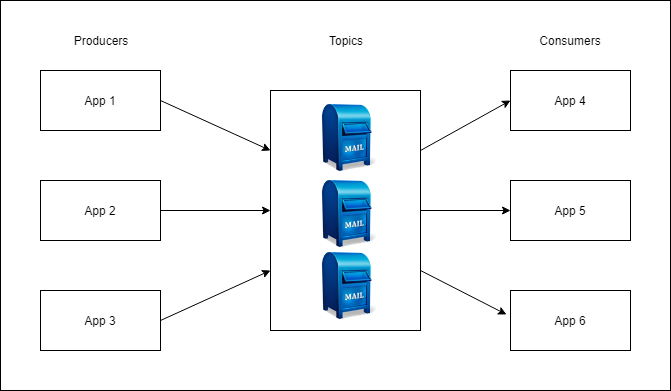
\includegraphics[scale=0.5,width=100mm]{./images/kafka-producrs-consumers-topics.png}
  \caption{Producers, Topics and Consumers}
  \label{fig:producers-topics-consumers}
\end{figure}

\subsection{Producers}

The role of a producer is to generate a message. This can be from any application, for example we could have a chat application that takes user input and sends messages to Kafka, alternatively we could have usage tracking on a user interface, a message is sent every time a user clicks a specific button. These are 2 completely different scenarios and that is exactly the point, Kafka does not discriminate where the information comes from. It is more concerned with how quickly and reliably it can get this data to the consumer.

There are 3 primary ways of sending messages to Kafka. The first is fire-and forget. With this approach we should not care what happens to the message after it has been sent because we have no guarantee that it has been received. Using this method it is likely that some messages will get lost. The second method is to send synchronously. Using this method we will be informed when Kafka has either stored the message or Kafka has thrown an error, such as no leader exception. The final method is to send asynchronously. Using this method we will not block our main thread. Our application can define a callback that will execute once Kafka has stored the message. In most situations asynchronous sending is proffered as it doesn't block our main thread for each message and still supports handling errors captured within our callback.

The producer has a number of configuration properties it can send along with the message, these will affect how the message will be sent. Some of these configuration parameters are outlined below

\begin{itemize}
  \item \textbf{acks} controls the level of replication.
  \item \textbf{buffer.memory} The total memory the producer will use to buffer messages waiting to be sent to the producer
  \item \textbf{compression.type} controls what compression to use. This can be snappy, gzip or lz4
  \item \textbf{retries} How many times our producer will retry sending a message before giving up
\end{itemize}

\subsection{Topics}

All messages that enter the system are organized into topics. Only consumers that are listening to certain topics will receive the messages that were published to that topic. Topics are stored in brokers. They are stored as a log on the file-system.

\subsection{Consumers}

As with the producers, a consumer can be just about any application imaginable. The consumer listens to topics for messages and needs to know how to interpret those messages. Because the messages can be in any format, from binary to JSON, it needs to know how handle them. One popular data serialization library is Apache Avro. It uses JSON for defining data types and protocols and serializes data in a compact binary format \cite{wiki:avro}.